% =========================================================
% CSC311 Final Project Report
% =========================================================

\documentclass[12pt]{article}

% ---------- Packages ----------
\usepackage[margin=1in]{geometry}
\usepackage{parskip}         % blank line between paragraphs, no indent
\usepackage{graphicx}
\usepackage{booktabs}
\usepackage{amsmath, amssymb}
\usepackage{siunitx}
\usepackage[hidelinks]{hyperref}
\usepackage{caption}
\usepackage{enumitem}
\usepackage{xcolor}
\usepackage{mathpazo}
\usepackage{float}

%--------- Headers and footers ------
\usepackage{fancyhdr}
\pagestyle{fancy}
\setlength{\headheight}{14.5pt}
\fancyhf{}
\fancyhead[L]{CSC311 Project Report}
\fancyhead[R]{3 Yellow 1 Brown}
\fancyfoot[C]{\thepage}

% ---------- Captions & Lists ----------
\captionsetup{font=small, labelfont=bf}
\setlist[itemize]{noitemsep, topsep=2pt}
\setlist[enumerate]{noitemsep, topsep=2pt}

\begin{document}

\begin{titlepage}
    \centering
    \vspace*{3cm}

    {\Large {CSC311: Introduction to Machine Learning \par}
    \vspace{1cm}

    {\Large {Project Report \par}
    \vspace{1cm}

    {\large \textit{Painting Classifier} \par}
    \vspace{3cm}

    {\large Submitted by \par}

    \vspace{0.5cm}
    {\large Thanh Nguyen, Justin Long, Shengdi Zhu, Yash Khanchandani \par}
    \vfill
    {\large University of Toronto\\Winter 2026\par}
\end{titlepage}
\clearpage
\setcounter{page}{1}

% =========================================================
\section{Data Exploration}
% =========================================================

The dataset contains 1686 survey responses, evenly distributed across three paintings (562 each): \textit{The Persistence of Memory}, \textit{The Starry Night}, and \textit{The Water Lily Pond}. Each response consists of 16 columns, including numerical ratings, Likert-scale responses, multi-select categorical questions, and free-text descriptions.

\subsection*{Numerical and Categorical Features}

We computed the mean and standard deviation of each feature, grouped by painting class. The raw Likert-scale responses (e.g., ``4 -- Agree'') were parsed to numeric values 1--5. Multi-valued categorical columns (room, companion, season) were converted to binary indicator variables: for example, the room column was split into five binary columns (Bathroom, Dining room, Office, Bedroom, Living room), where each column is 1 if the respondent selected that option and 0 otherwise.

Table~\ref{tab:eda} summarizes the features with the most significant differences in mean across paintings.

\begin{table}[H]
\centering
\caption{Selected feature means per painting class.}
\label{tab:eda}
\small
\begin{tabular}{lccc}
\toprule
\textbf{Feature} & \textbf{Persistence} & \textbf{Starry Night} & \textbf{Water Lily} \\
\midrule
Fall (season)        & 0.59 & 0.18 & 0.02 \\
Spring (season)      & 0.08 & 0.20 & 0.80 \\
Winter (season)      & 0.20 & 0.52 & 0.00 \\
Sombre (1--5)        & 3.91 & 2.76 & 1.64 \\
Calm (1--5)          & 2.65 & 3.91 & 4.47 \\
Uneasy (1--5)        & 3.85 & 2.11 & 1.36 \\
Content (1--5)       & 2.15 & 3.62 & 4.41 \\
Bedroom (room)       & 0.10 & 0.60 & 0.48 \\
Family members       & 0.21 & 0.61 & 0.69 \\
\bottomrule
\end{tabular}
\end{table}

Season features show strong separation: \textit{Fall} is a clear indicator of Persistence of Memory, \textit{Spring} for Water Lily Pond, and \textit{Winter} for Starry Night. The mood scores (Sombre, Uneasy, Calm, Content) form a gradient from the dark, unsettling Persistence of Memory to the serene Water Lily Pond. Room and companion choices also provide moderate separation.

We chose to drop the \textit{Willingness to Pay} feature. The raw responses contained extreme outliers (maximum of \$10\textsuperscript{30}), and after inspection, the feature primarily reflects the respondent's attitude toward art in general rather than which painting they are describing.

\subsection*{Text Feature Analysis}

Rather than using full NLP (e.g., TF-IDF with thousands of features), we identified \textit{painting-specific keywords} from the free-text responses. Using \texttt{find\_common\_words.py}, we computed the most frequent words in the ``Describe how this painting makes you feel'' column for each painting, after removing punctuation and common stop words. We selected words that appear frequently for one painting but rarely for the others:

\begin{itemize}
    \item \textbf{Persistence of Memory:} time (313), sad (87), clocks (71), melting (47), passing (26)
    \item \textbf{Starry Night:} calm (149), sky (72), night (61), awe (35), wonder (34)
    \item \textbf{Water Lily Pond:} happy (179), warm (44), nature (34), joyful (25), bright (24)
\end{itemize}

We repeated this analysis for the soundtrack and food text columns, yielding additional discriminative keywords. Each keyword was converted to a binary indicator (1 if the word appears in the response, 0 otherwise), using exact word matching after stripping punctuation.

\subsection*{Data Representation and Splitting}

The final feature set consists of 7 numerical features (emotion intensity, prominent colours, objects, and 4 parsed Likert scores), 14 categorical binary indicators (5 rooms, 5 companions, 4 seasons), and 56 keyword binary indicators (17 from feelings, 25 from soundtrack, 14 from food), for a total of 77 features. Missing numerical values are imputed with the training median; missing categorical values default to 0 (``did not select''). All features are z-normalized using training set statistics.

We evaluate all models using 5-fold stratified cross-validation (\texttt{random\_state=42}), which preserves the class balance in each fold and ensures every sample is predicted exactly once while held out. This provides an honest estimate of generalization performance.

% =========================================================
\section{Model Exploration}
% =========================================================

\subsection*{Logistic Regression}

We began with the hypothesis that textual responses are unreliable features, since each respondent's vocabulary and cultural knowledge varies drastically. To test this, we built a multinomial logistic regression (softmax classifier) using only the 21 numerical and categorical features, excluding all text-derived features.

Using \texttt{sklearn}'s \texttt{LogisticRegression} with the L-BFGS solver, we performed a grid search over the regularization parameter $C \in \{0.001, 0.01, 0.1, 1.0, 3.0, 5.0, 10.0\}$. The optimal value was $C = 3.0$, yielding a 5-fold CV accuracy of approximately 84.6\%. This confirmed that structured features alone carry strong predictive signal, establishing a solid baseline.

\subsection*{Gradient Boosting}

While logistic regression uses linear decision boundaries, some painting distinctions may require capturing non-linear feature interactions. For example, the combination ``Fall + high Sombre score'' is a much stronger indicator of \textit{The Persistence of Memory} than either feature alone. Gradient Boosting naturally captures such interactions through its sequential tree-building process, where each shallow decision tree can split on different feature combinations.

We first tested Gradient Boosting on the same 21 features, achieving approximately 86\% CV accuracy---a clear improvement over logistic regression. We then incorporated the keyword binary features from all three text columns (feelings, soundtrack, food), bringing the feature set to 77 dimensions. This further improved accuracy to approximately 89.7\%.


\subsection*{Naive Bayes}
To explore further, we evaluated Naive Bayes (NB) classifiers as a lightweight baseline. NB classifiers are, as shown in our lectures, well-suited for classification with features that can be assumed to be conditionally independent given the class labels. Since our dataset is a hybrid between binary indicator variables and continuous normalized features, with \textbf{70/77} of the dataset being \textbf{binary} and \textbf{7/77} being \textbf{numerical}, we investigated two variants of NB classifiers which would best capture the input data distribution.

\subsubsection*{Gaussian Naive Bayes}
We first experimented with the Gaussian NB. This was a natural approach because our features were \textbf{normalized} during pre-processing to have a mean of 0 and a variance of 1, and Gaussian NB assumes that the features follow a \textbf{Gaussian distribution}, which the normalized continuous features approximately follow. Using 5-fold stratified cross-validation, we tuned the hyperparameter \textit{var\_smoothing} and achieved a maximum CV accuracy of \textbf{81.08\%} with $var\_smoothing = 0.325$. The normalization of the dataset reduced the variance of each feature, hence the larger smoothing value.

\subsubsection*{Bernoulli Naive Bayes}
We experimented with Bernoulli NB as it is well-suited for unnormalized binary data. Bernoulli NB is specifically designed for binary features, representing each feature as a Bernoulli random variable, and \textbf{70/77} features in our dataset are binary. We hypothesized that the Bernoulli NB would be a stronger candidate because it captures binary data features more accurately. We also used \textbf{unnormalized} data to preserve the binary nature of the features. Using 5-fold stratified cross-validation, we achieved an accuracy of \textbf{85.74\%} - noticeably higher than the Gaussian NB. This was achieved with the smoothing hyperparameter $alpha=0.215$ and the threshold hyperparameter $binarize=0.0$ (which sets features greater than 0 equal to 1, and 0 otherwise).

\subsection*{The Ensembles}
We concluded the hyperparameter tuning portion of the models by comparing their accuracies and performance both individually and when incorporated into a majority vote ensemble with Gradient Boosting and Logistic Regression.

\begin{table}[H]
\centering
\caption{CV accuracy across individual models and the ensembles}
\label{tab:depth}
\begin{tabular}{ccc}
\toprule
\texttt{model} & CV Accuracy & Std \\
\midrule
\textbf{Gradient Boosting} & \textbf{0.8974} & \textbf{0.0055} \\
Logistic Regression & 0.8808 & 0.0044 \\
Gaussian Naive Bayes & 0.8108 & 0.0163 \\
Bernoulli Naive Bayes & 0.8547 & 0.0154 \\
Ensemble (Gaussian NB) & 0.8938 & 0.0069 \\
Ensemble (Bernoulli NB) & 0.8915 & 0.0081 \\
\bottomrule
\end{tabular}
\end{table}
Both ensemble accuracies were \textbf{below} the Gradient Boosting
model's standalone accuracy of \textbf{89.74\%}. Notably, the ensemble
incorporating Bernoulli NB (\textbf{89.15\%}) performed slightly worse than
the one incorporating Gaussian NB (\textbf{89.38\%}) despite
Bernoulli NB having a higher standalone accuracy. This is
because the ensemble uses a majority vote mechanism, and Bernoulli
NB was trained and optimized on \textbf{unnormalized} data, while Gradient
Boosting and Logistic Regression were trained on \textbf{normalized}
data. Furthermore, Bernoulli NB binarized the \textbf{7/77} features that were numerical, thereby losing the information about their magnitudes. The combination of these two factors frequently created conflicting outputs between the Bernoulli NB and the other two models, negatively impacting the majority-vote ensemble more than the Gaussian NB ensemble. As a result, we concluded that \textbf{Gradient Boosting} alone would be the strongest model for inference.

% --- Placeholder for teammates' models ---

% \subsection*{[Team member 3's model]}
% \textit{[To be filled in by team member.]}

% \subsection*{[Team member 4's model]}
% \textit{[To be filled in by team member.]}

% =========================================================
\section{Model Choice and Hyperparameters}
% =========================================================

\subsection*{Evaluation Methodology}

All models were evaluated using 5-fold stratified cross-validation with the same fold assignments (\texttt{StratifiedKFold}, \texttt{shuffle=True}, \texttt{random\_state=42}). We use \textbf{accuracy} as the evaluation metric. Since the dataset is perfectly balanced (562 samples per class), accuracy is not misleading and directly reflects per-class performance.

\subsection*{Hyperparameter Tuning}

For the Gradient Boosting classifier, we tuned three hyperparameters: \texttt{n\_estimators} (number of boosting rounds), \texttt{max\_depth} (maximum depth of each tree), and \texttt{learning\_rate} (shrinkage applied to each tree's contribution).

We performed an exhaustive grid search using five parallelized scripts \\(\texttt{hyperparameter\_search[1-5].py}), each covering a different range of \texttt{n\_estimators} from 100 to 800, with \texttt{max\_depth} $\in \{2, 3, 4, 5\}$ and \texttt{learning\_rate} $\in \{0.01, 0.03, 0.05, 0.07, 0.1, 0.15, 0.2\}$. The scripts were run concurrently on separate terminal instances using \texttt{joblib.Parallel} for within-script parallelization.

Tables~\ref{tab:depth}, \ref{tab:lr}, and \ref{tab:nest} show the CV accuracy when varying each hyperparameter while holding the others at their optimal values.

\begin{table}[H]
\centering
\caption{CV accuracy varying \texttt{max\_depth} (\texttt{n\_estimators}=200, \texttt{learning\_rate}=0.15).}
\label{tab:depth}
\begin{tabular}{ccc}
\toprule
\texttt{max\_depth} & CV Accuracy & Std \\
\midrule
\textbf{2} & \textbf{0.8974} & 0.0055 \\
3 & 0.8915 & 0.0109 \\
4 & 0.8855 & 0.0045 \\
5 & 0.8832 & 0.0058 \\
\bottomrule
\end{tabular}
\end{table}

\begin{table}[H]
\centering
\caption{CV accuracy varying \texttt{learning\_rate} (\texttt{n\_estimators}=200, \texttt{max\_depth}=2).}
\label{tab:lr}
\begin{tabular}{ccc}
\toprule
\texttt{learning\_rate} & CV Accuracy & Std \\
\midrule
0.01 & 0.8535 & 0.0220 \\
0.03 & 0.8790 & 0.0122 \\
0.05 & 0.8909 & 0.0083 \\
0.07 & 0.8920 & 0.0117 \\
0.10 & 0.8920 & 0.0081 \\
\textbf{0.15} & \textbf{0.8974} & 0.0055 \\
0.20 & 0.8950 & 0.0068 \\
\bottomrule
\end{tabular}
\end{table}

\begin{table}[H]
\centering
\caption{CV accuracy varying \texttt{n\_estimators} (\texttt{max\_depth}=2, \texttt{learning\_rate}=0.15).}
\label{tab:nest}
\begin{tabular}{ccc}
\toprule
\texttt{n\_estimators} & CV Accuracy & Std \\
\midrule
100 & 0.8926 & 0.0081 \\
150 & 0.8950 & 0.0052 \\
\textbf{200} & \textbf{0.8974} & 0.0055 \\
300 & 0.8950 & 0.0051 \\
400 & 0.8932 & 0.0026 \\
500 & 0.8909 & 0.0059 \\
\bottomrule
\end{tabular}
\end{table}

The optimal configuration is \texttt{n\_estimators}=200, \texttt{max\_depth}=2, \texttt{learning\_rate}=0.15, achieving a CV accuracy of \textbf{89.74\% $\pm$ 0.55\%}. Increasing tree depth beyond 2 leads to overfitting (accuracy decreases monotonically). Higher \texttt{n\_estimators} shows diminishing returns and slight degradation, indicating the model converges quickly with this learning rate. The learning rate of 0.15 sits at a sweet spot since lower values underfit (especially 0.01), while 0.20 slightly overshoots.

\subsection*{Confusion Matrix}

To understand the model's error patterns, we generated a confusion matrix using \texttt{matplotlib} and the function \texttt{cross\_val\_predict} from \texttt{sklearn}
(Figure~\ref{fig:cm}).

\begin{figure}[H]
\centering
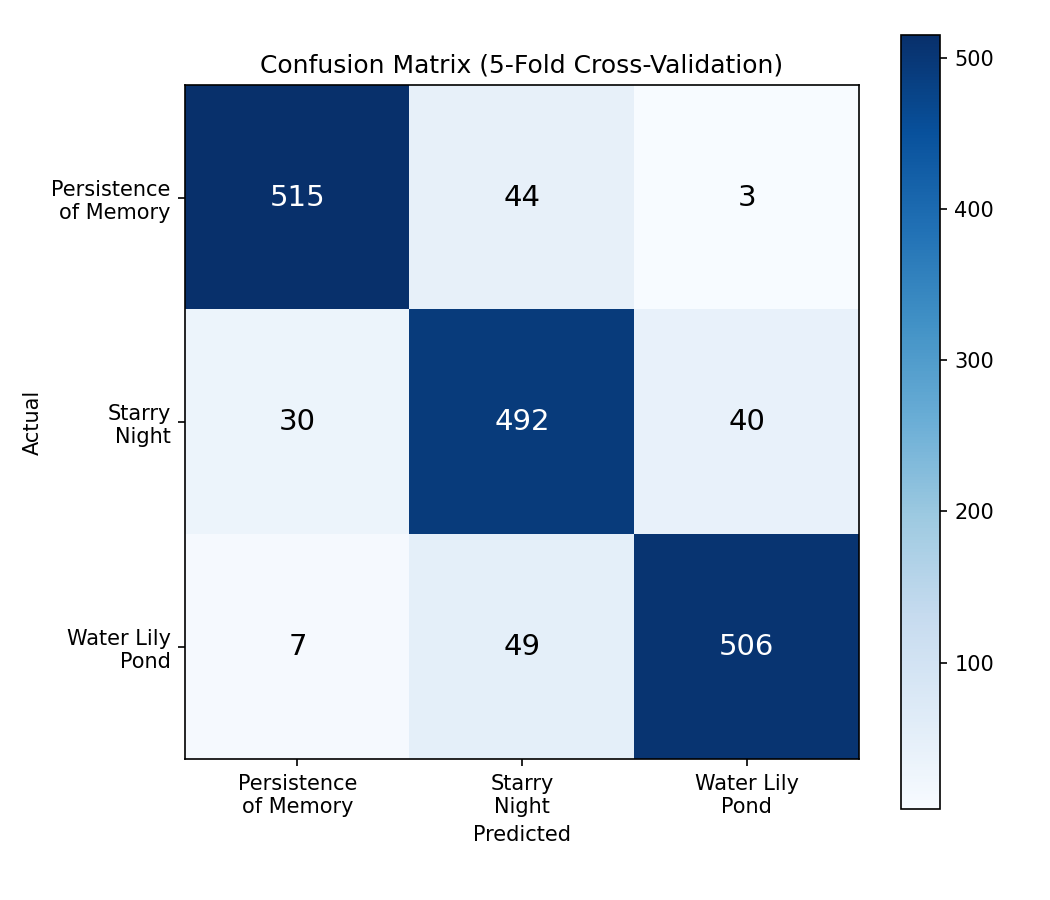
\includegraphics[width=0.65\linewidth]{confusion_matrix.png}
\caption{Confusion matrix from 5-fold cross-validation predictions.}
\label{fig:cm}
\end{figure}

The primary source of error is confusion between \textit{The Starry Night} and \textit{The Water Lily Pond} (89 of 173 total errors, or approximately 51\%). This is expected, as both paintings evoke calm, peaceful emotions, making them harder to distinguish on mood features alone. \textit{The Persistence of Memory} is well-separated due to its distinctly dark and uneasy characteristics.

\subsection*{ROC Curves}

We computed one-vs-rest ROC curves using cross-validated probability predictions (Figure~\ref{fig:roc}). The high AUC values (all above 0.96) indicate strong ranking ability across all classes. \textit{The Starry Night} has the lowest AUC (0.969), consistent with the confusion matrix showing it is the most frequently misclassified painting.

\begin{figure}[H]
\centering
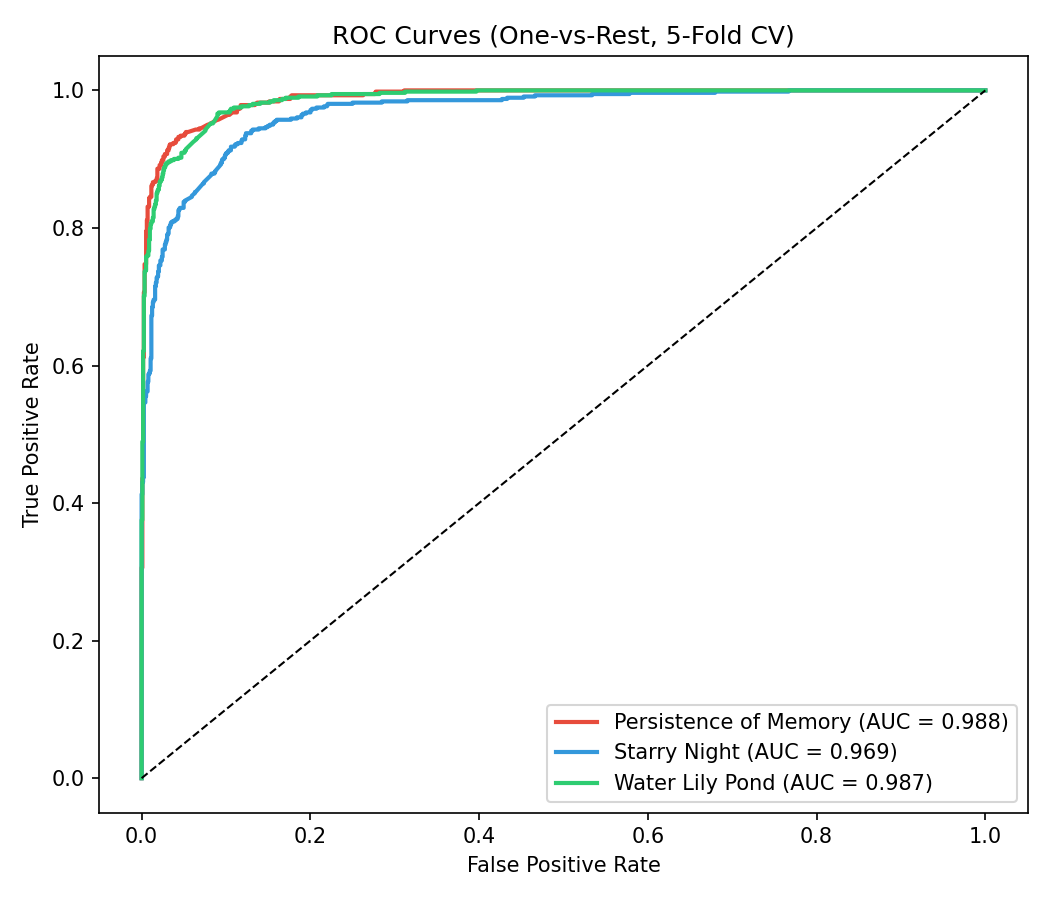
\includegraphics[width=0.65\linewidth]{roc_curves.png}
\caption{One-vs-rest ROC curves with AUC values from 5-fold cross-validation.}
\label{fig:roc}
\end{figure}

\subsection*{Final \texttt{pred.py} Implementation}

For the submitted \texttt{pred.py}, we implemented Gradient Boosting inference from scratch using only \texttt{numpy} and \texttt{pandas}. The 600 decision trees (200 rounds $\times$ 3 classes) were extracted from the trained \texttt{sklearn} model and saved to \texttt{gb\_model\_params.npz}. At inference time, each test sample is passed through all trees via a vectorized tree traversal function, accumulating \texttt{learning\_rate} $\times$ leaf values. The final prediction is the class with the highest accumulated score.

% =========================================================
\section{Prediction}
% =========================================================

We estimate that our model will achieve approximately \textbf{87\%} accuracy on the unseen test set.

Our 5-fold cross-validation accuracy on the training data is 89.7\%. We expect a drop of 2--3\% on the test set for the following reasons:

\begin{enumerate}
    \item \textbf{Distribution shift:} The test set is generated by TAs and instructors, who may use different vocabulary, have different cultural references, and possess different levels of art knowledge compared to students. Our keyword features were derived from student responses, and some keywords may not transfer to TA responses.

    \item \textbf{Keyword specificity:} The 56 keyword binary features are based on word frequencies in the training data. TAs may use synonyms or phrasing that our keyword set does not capture (e.g., ``sorrowful'' instead of ``sad'').

    \item \textbf{Structural features remain robust:} The numerical and categorical features (season, mood scores, room, companion) should transfer well, since the visual properties of the paintings do not change regardless of who views them. These features alone achieved 86\% accuracy.

    \item \textbf{Regularization:} The model uses shallow trees (\texttt{max\_depth}=2), limiting its capacity to memorize training-specific patterns. The monotonic accuracy decrease with deeper trees (Table~\ref{tab:depth}) confirms we are not overfitting.

    \item \textbf{Persistent confusion:} The confusion between \textit{The Starry Night} and \textit{The Water Lily Pond} is likely inherent to the paintings' shared aesthetic qualities and will persist regardless of the respondent population.
\end{enumerate}

% =========================================================
\section{Workload Distribution}
% =========================================================

\textbf{Thanh Nguyen:}
\begin{enumerate}
\item Computed the mean and standard deviation of numerical and categorical variables for data exploration.
\item Fine-tuned gradient boosting hyperparameters via parallelized exhaustive grid search.
\item Wrote the project report.
\end{enumerate}

\textbf{Yash Khanchandani:}
\begin{enumerate}
\item Fine-tuned the hyperparameters of Logistic Regression, Gaussian Naive Bayes, and Bernoulli Naive Bayes, using an exhaustive grid search.
\item Tested predictions between the validated individual models their majority-vote ensembles to determine the most optimal model to be used for inference.
\item Wrote the Naive Bayes and Ensemble model explorations in the project report.
\end{enumerate}

\textbf{[Team member 3]:} \textit{[To be filled in by team member.]}

\textbf{[Team member 4]:} \textit{[To be filled in by team member.]}

\end{document}
